%%%%%%%%%%%%%%%%%%% Frame de garde
\begin{frame}[plain]
    \begin{center}
        \vspace{1cm}
        \textcolor{ceruleanblue}{\Large \bfseries Embedded Convex Optimization for Control of Synchronous machines} \\
        \vspace{0.8cm}
        {\normalsize Hiba HOUMSI}\\
        \vspace{0.3cm}
        {\textbf{\textcolor{brown!130}{Supervisors:}} Paolo Massioni, Federico Bribiesca-Argomedo, Romain Delpoux}\\
        \vspace{0.5cm}
        {\small
        \textbf{\textcolor{brown!130}{Jury Committee:}}\\
        \vspace{0.2cm}
        \begin{tabular}{@{}llll@{}}
            \textbf{Examiner:} & Delphine Riu & Professor & Grenoble INP-Ense3 \\
            \textbf{Reviewers:} & Giorgio Valmorbida & Professor & CentraleSupélec \\
                               & Václav Šmídl &  Professor &  CTU Prague \\
            \textbf{Invited:} & Lubin Kerhuel & PhD Engineer & Microchip, inc.
        \end{tabular}
        }\\
        \vspace{0.6cm}
        %{\footnotesize Ampère laboratory, INSA Lyon, France}
        %\vspace{0.2cm}
        {\footnotesize PhD Defense, \today}

        \vspace{0.1cm}
        \begin{figure}[htbp]
        \begin{center}
        \href{http://www.ampere-lab.fr/}{
\includegraphics[height = 1cm]{pictures/logo/logoAMPERE}}
        \href{https://www.insa-lyon.fr/}{
\includegraphics[height = 1cm]{pictures/logo/INSA}}
        
\includegraphics[height=1cm]{pictures/logo/CNRS}
        
\includegraphics[height=1cm]{pictures/logo/UDL}
        
\includegraphics[height=1cm]{pictures/logo/Centrale}
        
\includegraphics[height=1cm]{pictures/logo/Lyon1}
        \end{center}
        \end{figure}
    \end{center}
\end{frame}
%%%%%%%%%%%%%%%%%%% Frame de Venn diagram
\section{Problem statement}
\begin{frame}{Problem Statement}{The embedded approach}
         \only<1->{
            Implement \textcolor{Red}{advanced control laws synthesis} on \textcolor{ceruleanblue}{low-cost hardware} to drive \textcolor{Green}{real-world systems}.
     }
     \vspace{-0.5cm}
     \begin{figure}
        %\centering
        \begin{tikzpicture}[scale= 0.8]
        \coordinate (origin) at (0,0);
        \only<2->{% Green circle - appears from slide 4 onwards
            \draw [Green, line width=0.8mm](0,-1.5) circle (2);
            \node at (0,-2.5) {\textcolor{Green}{\shortstack{Control \\ Application}}};
            %\node at (-5,-3) {\includegraphics[width=2.5cm]{pictures/PMSM.eps}};
            \node at (-5,-5) {\shortstack{Permanent magnet \\ synchronous machines}};
            \draw [Green, line width=0.6mm, dashed, ->] (-0,-3.5) to[bend left=15] (-3,-5);
        }
        \only<3->{% Red circle - persistent from slide 2 onwards
            \draw [red,line width=0.8mm] (-1.3,0) circle (2);
            \node at (-1.8,1) {\textcolor{red}{\shortstack{Convex \\ Optimization}}};
           % \node at (-5.5,2) {\includegraphics[width=2.5cm]{pictures/Robust_control_law.eps}};
            %\node at (-8.5,2) {\includegraphics[width=2.5cm]{pictures/Robust_control_law.eps}};
            %\node at (-5.5,0) {\shortstack{Feedback \\ control}};
            %\node at (-8.5,0) {\shortstack{Trajectory \\ generation}};
            \node at (-5.5,2) {\shortstack{Feedback \\ control}};
            \node at (-8.5,2) {\shortstack{Trajectory \\ generation}};
            \draw [red, line width=0.6mm, dashed, ->] (-2,2) to[bend right=15] (-4,2);
        }
        \only<4->{% Blue circle - appears from slide 3 onwards
            \draw [ceruleanblue,line width=0.8mm] (1.3,0) circle (2);
            \node at (1.7,1) {\textcolor{ceruleanblue}{\shortstack{Embedded \\ systems}}};
            %\node at (5,1) {\includegraphics[width=2.5cm]{pictures/muC.eps}};
            %\node at (5,-1) {\shortstack{Microcontrollers \\ DSP}};
            \node at (5,1) {\shortstack{Microcontrollers \\ DSP \\ $\sim 5 \$ $/unit}};
            \draw [ceruleanblue, line width=0.6mm, dashed, ->] (2,2) to[bend left=15] (4.5,2);
        }
        \path[use as bounding box] (-10,-5) rectangle (10,3);% Invisible bounding box to maintain consistent tikzpicture size
        \end{tikzpicture}
     \end{figure}
\end{frame}

%%%%%%%%%%%%%%%%%%% Control engineer approach Hybrid offline online approach 
 \begin{frame}{Problem Statement}{The embedded approach}
    \begin{center}
    \only<1>{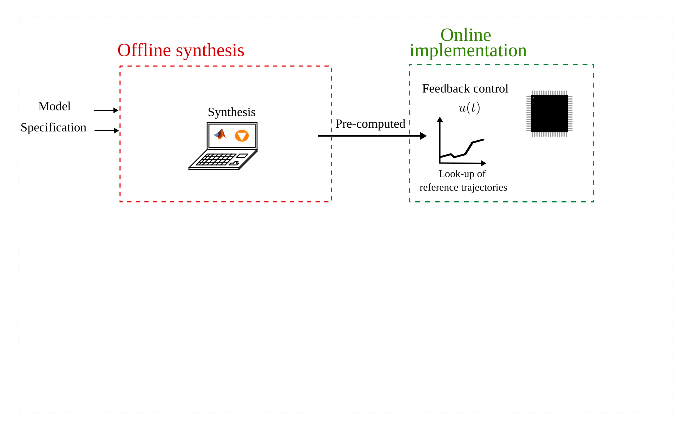
\includegraphics[trim={0cm 0cm 0cm 0cm},clip,width=0.9\framewidth]{pictures/online_offline1.eps}
    }
    %\only<2>{\includegraphics[trim={0cm 0cm 0cm 0cm},clip,width=0.9\framewidth]{pictures/online_offline_ink_trajec1.eps}
    %}
    \only<2>{
    \vspace{-0.3cm}    
    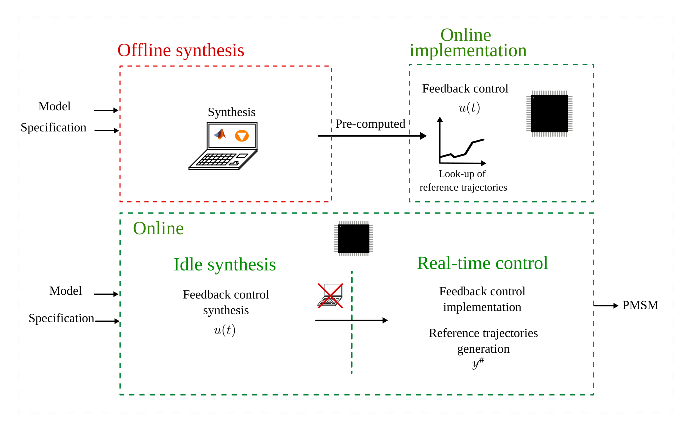
\includegraphics[trim={0cm 0cm 0cm 0cm},clip,width=0.9\framewidth]{pictures/online_offline2.eps}
    }
    \end{center}
 \end{frame}
%%%%%%%%%%%%%%%%%%% Frame PMSM is widely used
\begin{frame}{Problem Statement}
    Permanent Magnet Synchronous Motors (PMSM)
    \begin{center}
        Widely used in industry
    \end{center}
\vspace{-.5cm}
\begin{columns}[t]
    \begin{column}{0.33\textwidth}
    \begin{center}
        \only<1->{
        Automotive\\
        \vspace{.5cm}
        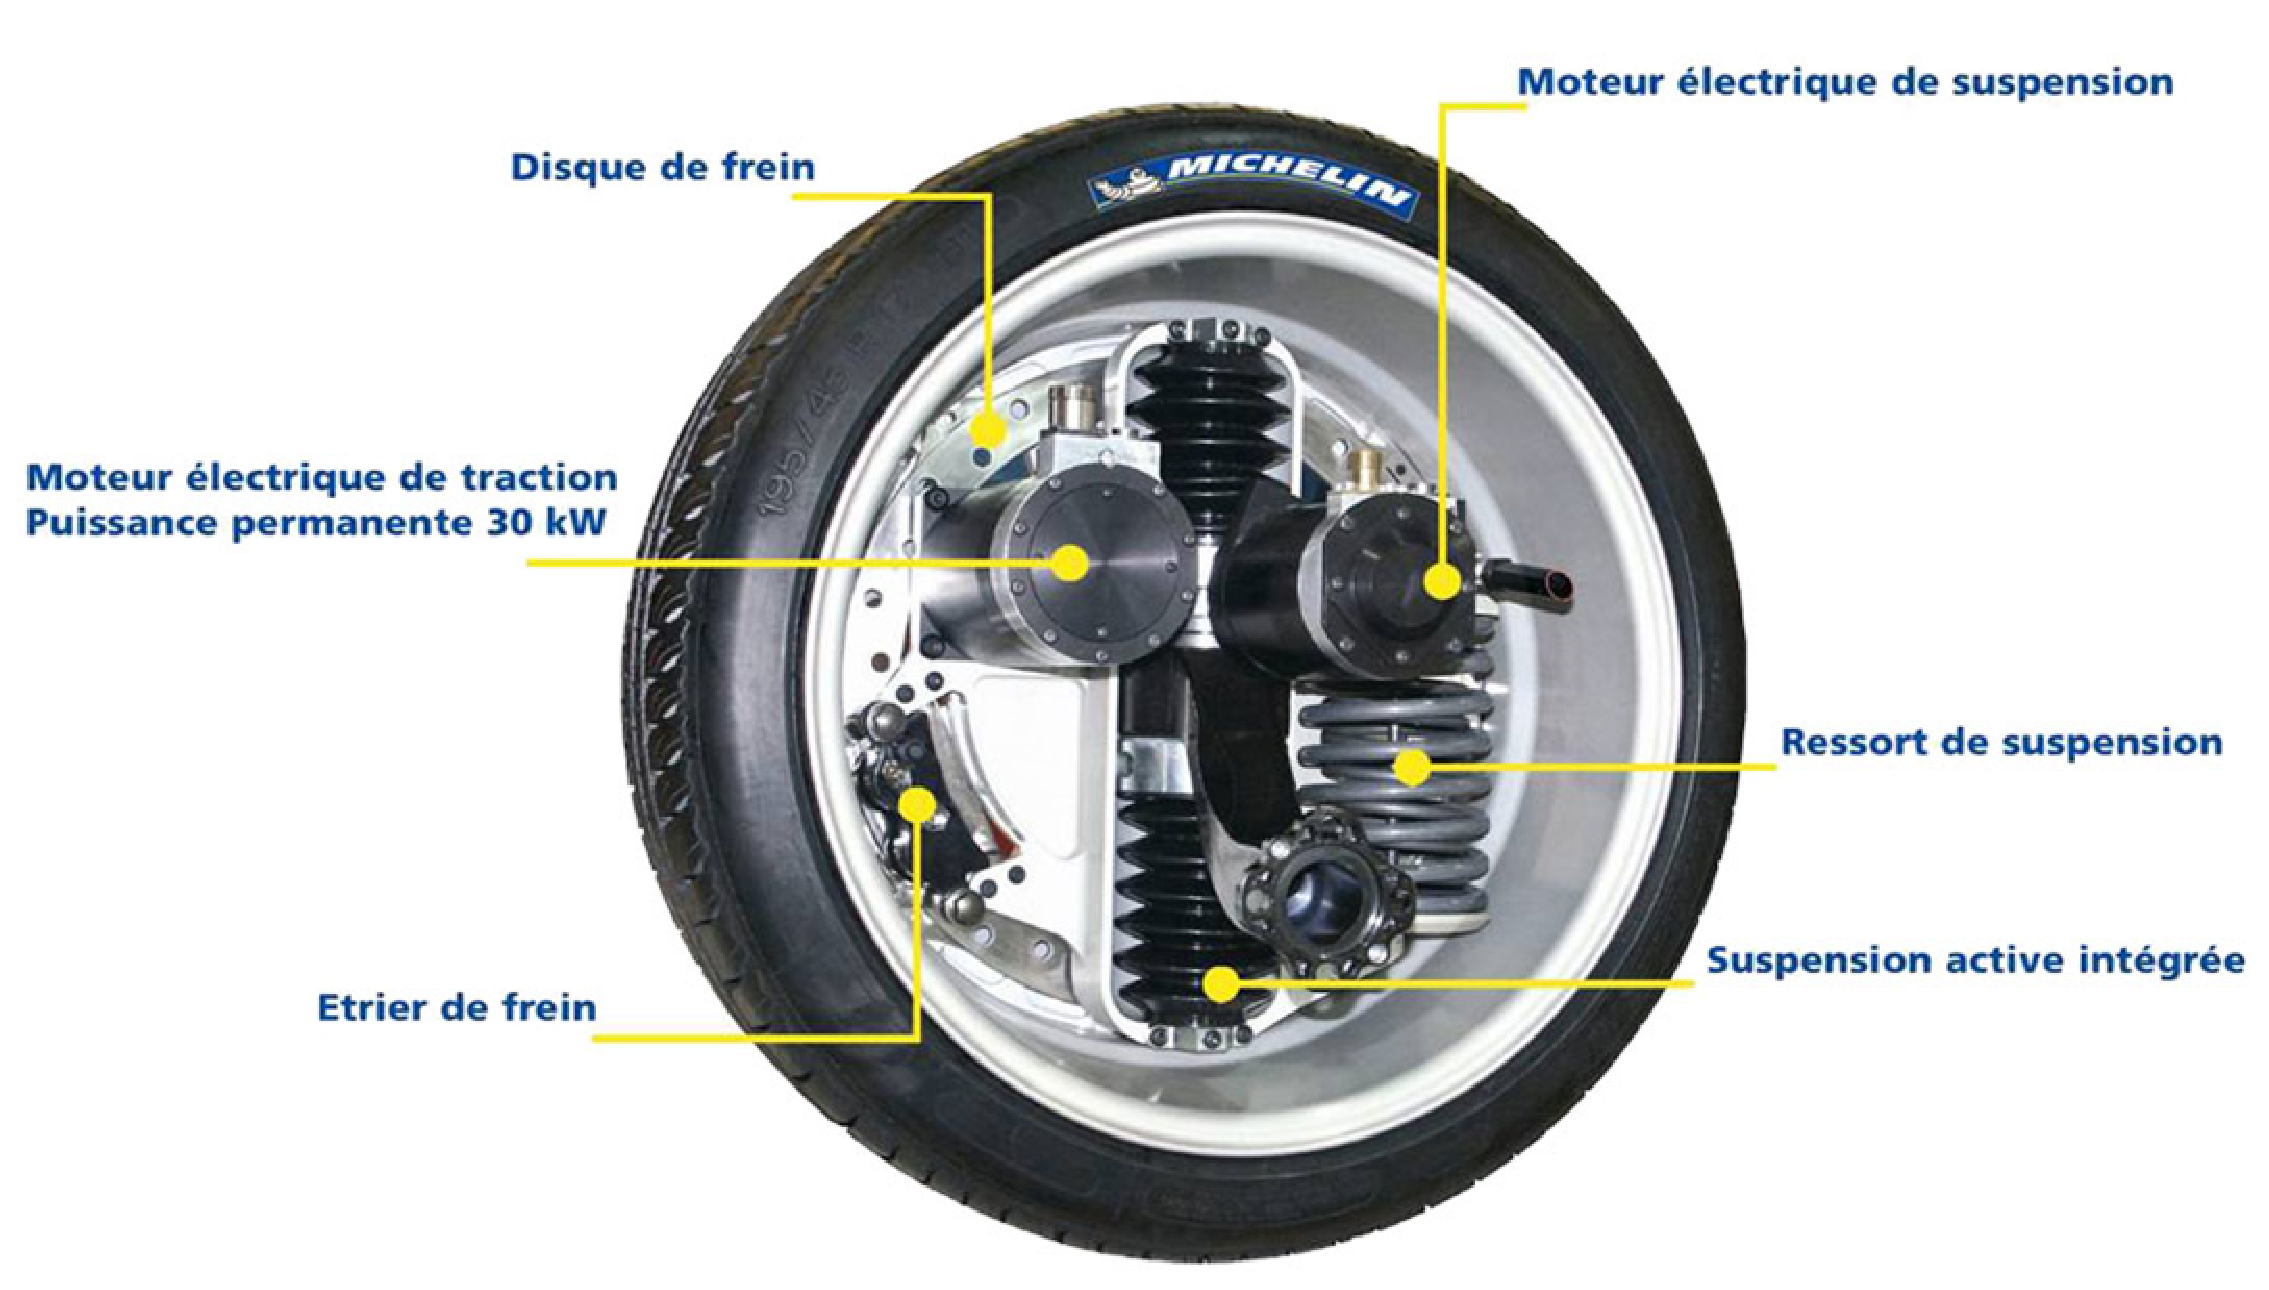
\includegraphics[width=0.8\textwidth]{pictures/Michelin.eps}
        }
    \end{center}
    \end{column}
%
    \begin{column}{0.33\textwidth}
    \begin{center}
    \only<2->{
        Robotics\\
        \vspace{.5cm}
        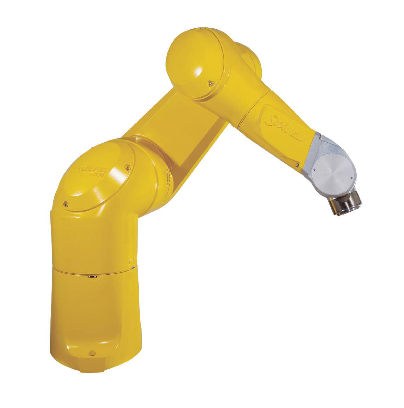
\includegraphics[width=0.8\textwidth]{pictures/TX90.eps}
    }
    \end{center}
\end{column}
    \begin{column}{0.33\textwidth}
        \begin{center}
        \only<3->{
        Power generation
        \vspace{.5cm}
        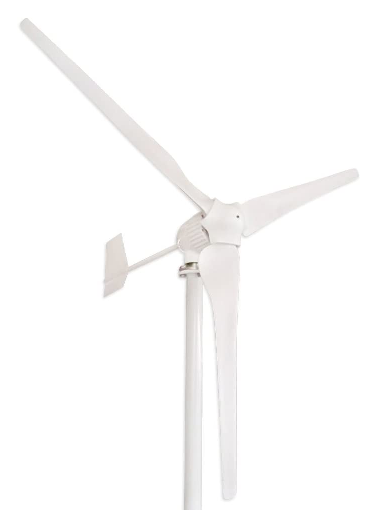
\includegraphics[width=.5\textwidth]{pictures/eolienne.eps}}
        \end{center}
    \end{column}
\end{columns}
    \only<4>{
    \vspace{.5cm}
    \alert{Goal: control torque and speed, while minimizing losses, taking into consideration the physical limitations.}}
\end{frame}
%%%%%%%%%%%%%%%%%%% Frame Park and Clarke transformations
\begin{frame}{Problem statement}{Simple representation of 3-phase PMSM}
    \begin{figure}
    \begin{tikzpicture}[scale=1.2]
    \tikzstyle{axis}=[thick,->]    % Styles
    \tikzstyle{coil}=[decoration={aspect=0.2, segment length=1mm, amplitude=3mm,coil},decorate,opacity=0.9]
    \tikzstyle{vector}=[->, thick]
    % ========== LEFT PART: 3D PMSM Representation ==========
    \only<1->{
    \begin{scope}[shift={(1,1)},scale=0.8]
        \coordinate (O) at (0,0);% Origin
        \fill[gray!40,rotate=50] (-0.8,-0.25) rectangle (0.8,0.25); % Draw rotor (rectangular, uniform light gray)
        \draw[thick,rotate=50] (-0.8,-0.25) rectangle (0.8,0.25);
        % Phase a axis (horizontal, towards front)
        \begin{scope}
            \draw[axis,black!70] (O) -- (0:2.8);
            \node at (0:3.0) {$a$};
            % Coil
            \draw[coil] (0:1.8) -- (0:2.2);
            % Voltage arrow (parallel to coil, 0.5cm offset below)
            \draw[vector,red] (1.8,-0.5) -- (2.2,-0.5) node[midway,below] {$v_{a}$};
            % Current arrow (on axis, closer to center)
            \draw[vector,blue] (1.1,0) -- (1.5,0) node[midway,below] {$i_{a}$};
        \end{scope}
        % Phase b axis (120 degrees)
        \begin{scope}[rotate=120]
            \draw[axis,black!70] (O) -- (0:2.8);
            \node at (0:3.0) {$b$};
            % Coil
            \draw[coil] (0:1.8) -- (0:2.2);
            % Voltage arrow (parallel to coil, 0.5cm offset below)
            \draw[vector,red] (1.8,-0.5) -- (2.2,-0.5) node[midway,right] {$v_{b}$};
            % Current arrow (on axis, closer to center)
            \draw[vector,blue] (1.1,0) -- (1.5,0) node[midway,below] {$i_{b}$};
        \end{scope}
        % Phase c axis (240 degrees)
        \begin{scope}[rotate=240]
            \draw[axis,black!70] (O) -- (0:2.8);
            \node at (0:3.0) {$c$};
            % Coil
            \draw[coil] (0:1.8) -- (0:2.2);
            % Voltage arrow (parallel to coil, 0.5cm offset below)
            \draw[vector,red] (1.8,-0.5) -- (2.2,-0.5) node[midway,left] {$v_{c}$};
            % Current arrow (on axis, closer to center)
            \draw[vector,blue] (1.1,0) -- (1.5,0) node[midway,right] {$i_{c}$};
        \end{scope}
        % Rotor angle theta_r
        \draw[thick,red] (O) -- (50:1.3) ; % node[midway,above,sloped,inner sep=1pt] {$\mathcal{N}$};
        \draw[-{Stealth[length=2mm]},thick,blue] (0.6,0) arc (0:50:0.6);
        \node at (25:1.2) {$\theta_r$};
        % Rotation indication
        \draw[-{Stealth[length=3mm]},thick,gray,dashed] (20:1.8) arc (20:80:1.8);
    \end{scope}
    % Label for left part
    \node at (1,-1.5) {\textbf{Static 3-coordinate system}};
    }
    % ========== RIGHT PART: d-q Frame Detail ==========
    \only<2>{
    \begin{scope}[shift={(7,1)},scale=0.8]
        \coordinate (C) at (0,0);
        % d-q axes
        \draw[axis,black!70,thick] (C) -- (50:3.5) node[anchor=south west] {$d$};
        \draw[axis,black!70,thick] (C) -- (140:3.5) node[anchor=south east] {$q$};
        % Angle theta_r from horizontal to d-axis
        \draw[-{Stealth[length=2mm]},thick,red] (0.8,0) arc (0:50:0.8);
        \node at (25:1.1) {$\theta_r$};
        \draw[axis,gray,dashed] (C) -- (0:1.2);
        \node at (0:1.4) {$\alpha$};
        % d-axis circuit (along d-axis)
        \begin{scope}[rotate=50]
            % Inductance L_d (coil)
            \draw[coil] (1.5,0) -- (2.0,0);
            \node at (1.75,0.5) {\small $L_d$};
            % Current arrow (on axis, further from coil)
            \draw[vector,blue] (2.1,0) -- (2.5,0) node[midway,below] {\small $i_d$};
            % Voltage arrow (at same height as coil)
            \draw[vector,red] (1.6,-0.5) -- (2,-0.5) node[midway,below=3pt] {\small $v_d$};
        \end{scope}
        % q-axis circuit (along q-axis)
        \begin{scope}[rotate=140]
            % Inductance L_q (coil)
            \draw[coil] (1.5,0) -- (2.0,0);
            \node at (1.75,0.5) {\small $L_q$};
            % Current arrow (on axis, further from coil)
            \draw[vector,blue] (2.6,0) -- (3.0,0) node[midway,below] {\small $i_q$};
            % Voltage arrow (at same height as coil)
            \draw[vector,red] (1.5,-0.5) -- (2 ,-0.5) node[midway,above=3pt] {\small $v_q$};
        \end{scope}
        % Rotor flux indication
        \draw[-{Stealth[length=3mm]},thick,red] (C) -- (50:1.2);
        \node[red] at (75:0.5) {$\phi_f$};
    \end{scope}
    % Label for right part
    \node at (7,-1.5) {\textbf{Rotating 2-coordinate system}};

    % Curved arrow showing transformation between the two systems
    \draw[-{Stealth[length=3mm]},thick,blue!70,line width=1.2pt]
        (3.2,0.31) to[out=-20,in=-160] (4.8,0.31);
    \node[align=center,fill=white,inner sep=2pt] at (4,-0.51)
        {\small \textbf{Park \& Clarke}\\ \small \textbf{transformation}};
    }
\end{tikzpicture}
    \end{figure}
\end{frame}
%%%%%%%%%%%%%%%%%%%%%%%%%%%%% Model of  the PMSM

\begin{frame}{Model of the PMSM}
    The nonlinear model of the system in the dq frame can  be represented as
 \begin{eqnarray*}
         L_d \frac{di_d}{dt} &=& v_d - Ri_d \textcolor{red}{+p L_q\omega i_q}, \\
         L_q\frac{di_q}{dt} &=& v_q -Ri_q \textcolor{red}{-pL_d\omega i_d} -p \phi_f\omega, \\
         J\frac{d\omega}{dt} &=&  \tau_{em}  - f\omega \textcolor{violet}{-\tau_l}.
     \end{eqnarray*}
     \pause
The system is subject to physical constraints:
    \begin{eqnarray*}
        & i_{dq}^\top i_{dq} - i_{max}^2 \leqslant 0, \\
        & v_{dq}^\top v_{dq} - v_{max}^2 \leqslant 0 ,  \\
        &\tau_{em} = \frac{3}{2}p \big( \phi_f +  (L_d - L_q) i_d \big) i_q.
    \end{eqnarray*}
\end{frame}
\begin{frame}{Problem statement}{System constraint}
    \begin{columns}
    \begin{column}{0.4\framewidth}
         \begin{eqnarray*}
            &\tikz[remember picture,baseline=(idqeq.base)]{\node[inner sep=0pt](idqeq){$i_{dq}^\top i_{dq} - i_{max}^2 \leqslant 0$};}\\
            \only<1-2>{&  \tikz[remember picture,baseline=(vdqeq.base)]{\node[inner sep=0pt](vdqeq){$v_{dq}^\top v_{dq} - v_{max}^2\leqslant 0$,};} \\}
            \only<3-4>{&  \tikz[remember picture,baseline=(vdqeq.base)]{\node[inner sep=0pt,align=center](vdqeq){$\textcolor{orange}{A(\omega)} i_d^2 + \textcolor{orange}{B(\omega)}i_di_q + \textcolor{orange}{C(\omega)}i_q^2+$ \\ $ \textcolor{orange}{D(\omega)}i_d + \textcolor{orange}{E(\omega)}i_q + \textcolor{orange}{F(\omega)} \leqslant 0$};} \\}
            \only<1-3>{& \tikz[remember picture,baseline=(taueq.base)]{\node[inner sep=0pt](taueq){$\tau_{em} - \frac{3}{2}p \big( \phi_f +  (L_d - L_q) i_d \big) i_q= 0.$}; }}
            \only<4>{& \tikz[remember picture,baseline=(taueq.base)]{\node[inner sep=0pt](taueq){$\textcolor{red}{\tau_{em}} - \frac{3}{2}p \big( \phi_f +  (L_d - L_q) i_d \big) i_q= 0.$}; }}
         \end{eqnarray*}
         \tikz[remember picture,overlay] {
            \only<1>{\draw[dashed,very thick,rounded corners,blue] ([xshift=-0.1cm,yshift=0.2cm]idqeq.north west) rectangle ([xshift=0.1cm,yshift=-0.08cm]idqeq.south east);}
            \only<2>{\draw[dashed,very thick,rounded corners,orange] ([xshift=-0.1cm,yshift=0.1cm]vdqeq.north west) rectangle ([xshift=0.1cm,yshift=-0.08cm]vdqeq.south east);}
            \only<3>{\draw[dashed,very thick,rounded corners,orange] ([xshift=-0.1cm,yshift=0.1cm]vdqeq.north west) rectangle ([xshift=0.1cm,yshift=-0.08cm]vdqeq.south east);}
            \only<4>{\draw[dashed,very thick,rounded corners,red] ([xshift=-0.1cm,yshift=0.1cm]taueq.north west) rectangle ([xshift=0.1cm,yshift=-0.08cm]taueq.south east);}
            }
    \end{column}
    \begin{column}{0.6\framewidth}
    \centering
     \only<1>{
        Current constraint in the $i_{dq}$ frame
        \centering
        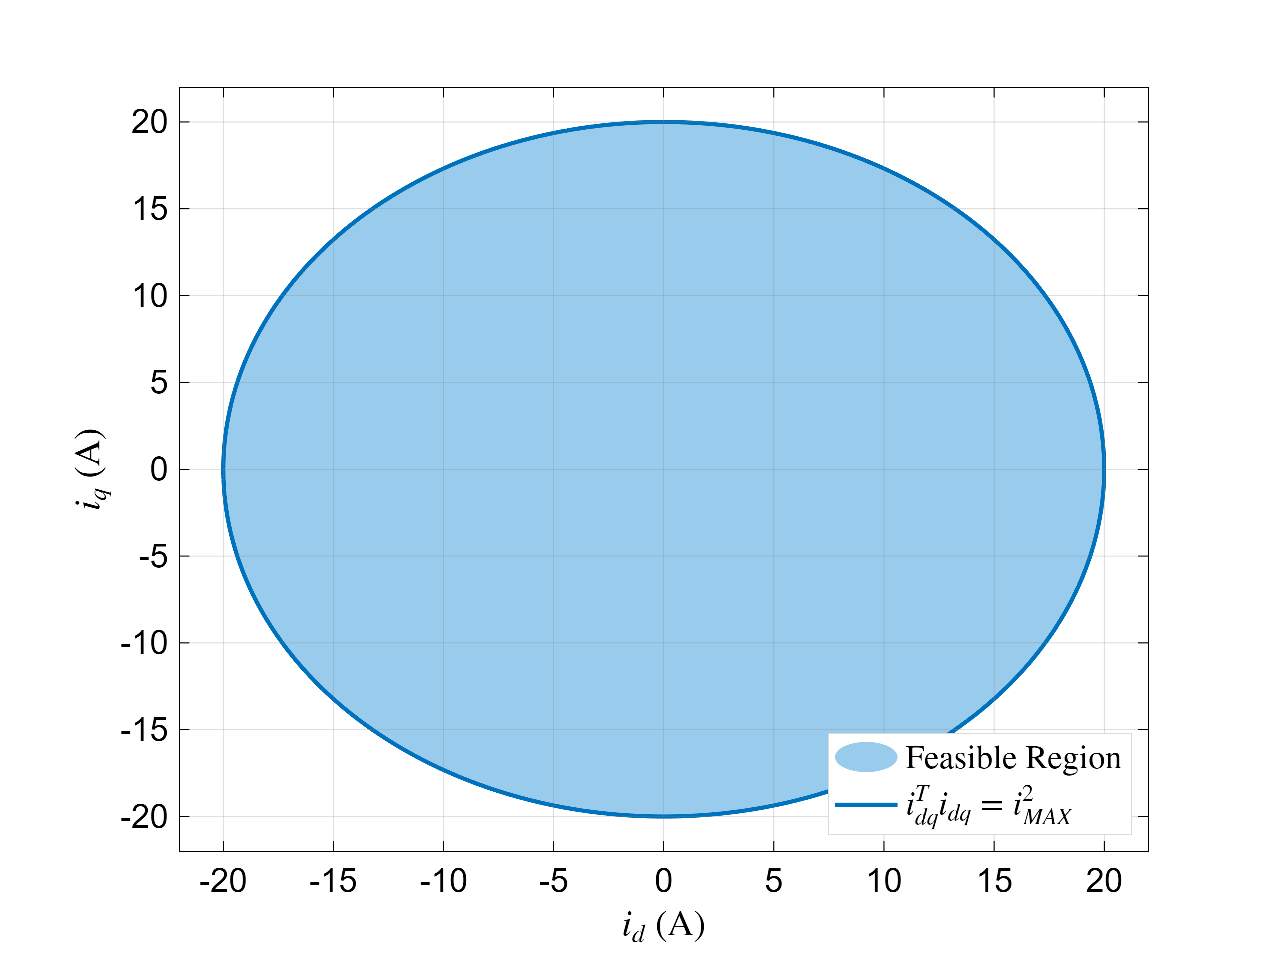
\includegraphics[width=7cm]{pictures/current_constraint_cost.eps}
     }
     \only<2>{
        Voltage constraint in the $i_{dq}$ frame
         \begin{eqnarray*}
            \cancel{L_d \frac{di_d}{dt}} &=& v_d - Ri_d +p L_q\omega i_q = 0, \\
            \cancel{L_q\frac{di_q}{dt}} &=& v_q -Ri_q -pL_d\omega i_d -p \phi_f\omega = 0,
       \end{eqnarray*}
     }
     \only<3>{
     \begin{center}
         \animategraphics[loop,controls,width=1\textwidth]{10}{eps_frames_voltage_animation_filled/frame_}{000}{040}
      \end{center}
     }
     \only<4>{
        Torque constraint in the $i_{dq}$ frame
      \begin{center}
          \animategraphics[loop,controls,width=1\textwidth]{10}{eps_frames_voltage_animation_torque/frame_}{000}{040}
      \end{center}
     }
    \end{column}
    \end{columns}
\end{frame}

\begin{frame}{Problem statement}%{To sum up}
\only<1->{
    \vspace{-0.3cm}
    \textbf{Goals:}
   % \vspace{0.2cm}
    %\hspace{+0.2cm}
    \begin{enumerate}
        \item[\textcolor{Cyan4}{\textbf{Part 1:}}] \textcolor{Cyan4}{Optimal currents $i_d^\#$, $i_q^\#$ to produce desired torque $\tau_{em}$ and speed $\omega$ }
        \only<2->{\item[\textcolor{Magenta4}{\textbf{Part  2:}}] \textcolor{Magenta4}{Embedded closed-loop control synthesis}}
        \only<3->{\item[\textcolor{blue}{\textbf{Part 3:}}] \textcolor{blue}{New control apporachs}}
    \end{enumerate}
}
\vspace{+0.1cm}
\begin{columns}[T]
    \begin{column}{0.5\textwidth}
        \tikz[remember picture,baseline=(optimalprob.base)]{\node[inner sep=5pt,align=left](optimalprob){\begin{minipage}{\textwidth}
        \textbf{\textcolor{Cyan4}{Part1: Optimal references}}
      \begin{center}
          \animategraphics[loop,autoplay,width=0.7\textwidth]{10}{eps_frames_voltage_animation_torque/frame_}{000}{040}
      \end{center}
        \only<1->{\small Output: $i_d^{\#}(\omega, \tau_{em})$, $i_q^{\#}(\omega, \tau_{em})$}
        \end{minipage}};}
        \tikz[remember picture,overlay] {
            \only<1>{\draw[dashed,very thick,rounded corners,Cyan4] ([xshift=-0.1cm,yshift=0.2cm]optimalprob.north west) rectangle ([xshift=0.1cm,yshift=-0.08cm]optimalprob.south east);}
        }
    \end{column}
    \begin{column}{0.5\textwidth}
    \only<2->{
        \tikz[remember picture,baseline=(controlprob.base)]{\node[inner sep=5pt,align=left](controlprob){\begin{minipage}{\textwidth}
        \textbf{\textcolor{Magenta4}{Part 2: Embedded closed-loop control synthesis}}
        
    %      \begin{eqnarray*}
    %      L_d \frac{di_d}{dt} &=& v_d - Ri_d +p L_q\omega i_q, \\
    %      L_q\frac{di_q}{dt} &=& v_q -Ri_q -pL_d\omega i_d -p \phi_f\omega, \\
    %      J\frac{d\omega}{dt} &=& \tau_{em}  -f\omega -\tau_l.
    %  \end{eqnarray*}
        \vspace{0.3cm} \textbf{Find} $u(t) = Kx(t)$ such that:
        \begin{itemize}
            \item Tracks $i_d^\#$, $i_q^\#$ trajectories
            \item Stable, easy-to-tune
            \item minimise the energy consumption
        \end{itemize}
        \end{minipage}};}
        \tikz[remember picture,overlay] {
            \only<2>{\draw[dashed,very thick,rounded corners,Magenta4] ([xshift=-0.1cm,yshift=0.2cm]controlprob.north west) rectangle ([xshift=0.1cm,yshift=-0.08cm]controlprob.south east);}
        }}
            \only<3->{
                \vspace{+0.3cm}
        \tikz[remember picture,baseline=(controlprob2.base)]{\node[inner sep=5pt,align=left](controlprob2){\begin{minipage}{\textwidth}
        \textbf{\textcolor{blue}{Part 3: Other closed-loop control strategies}}
        
    %      \begin{eqnarray*}
    %      L_d \frac{di_d}{dt} &=& v_d - Ri_d +p L_q\omega i_q, \\
    %      L_q\frac{di_q}{dt} &=& v_q -Ri_q -pL_d\omega i_d -p \phi_f\omega, \\
    %      J\frac{d\omega}{dt} &=& \tau_{em}  -f\omega -\tau_l.
    %  \end{eqnarray*}
        \vspace{+0.3cm}\textbf{Find} $u(t) = K(x(t))$ such that:
        \begin{itemize}
            \item Robust to measurement noise
            \item Robust to parametric uncertainty
        \end{itemize}
        \end{minipage}};}
        \tikz[remember picture,overlay] {
            \only<3>{\draw[dashed,very thick,rounded corners,blue] ([xshift=-0.1cm,yshift=0.2cm]controlprob2.north west) rectangle ([xshift=0.1cm,yshift=-0.08cm]controlprob2.south east);}
        }}
    \end{column}
\end{columns}
% Big frame encompassing both Problem 1 and 2 to show they are embedded in DSP
\tikz[remember picture,overlay] {
    \only<4>{
        \draw[dashed,ultra thick,rounded corners,red] ([xshift=0cm,yshift=0cm]optimalprob.north west) rectangle ([xshift=0cm,yshift=-0.5cm]optimalprob.south -| controlprob.east);
        \node[red,anchor=south east,font=\small\bfseries] at ([xshift=-0.1cm,yshift=-0.5cm]optimalprob.south -| controlprob.east) {Embedded};
    }
}
\only<3>{
\vspace{0.3cm}
\begin{center}
\tikz[remember picture,baseline=(embedprob.base)]{\node[inner sep=8pt,align=center](embedprob){%
\textbf{\textcolor{red}{Embedded}} Embedded implementation on \textcolor{red}{microcontrollers/DSP} ($\sim 5\$$/unit)};}
\tikz[remember picture,overlay] {
    \draw[dashed,very thick,rounded corners,red] ([xshift=0cm,yshift=0cm]embedprob.north west) rectangle ([xshift=0.1cm,yshift=-0.08cm]embedprob.south east);
}
\end{center}
}
\end{frame}

\begin{frame}{Outline}
    %%% loi de commande en boucle fermee
    %    \vspace{-0.3cm}
    \textbf{Objectives:}
    \vspace{0.2cm}
    \begin{enumerate}
        \item[\textcolor{Cyan4}{\textbf{ Part 1:}}] \textcolor{Cyan4}{\textbf{Optimal currents $i_d^\#$, $i_q^\#$ to produce desired torque $\tau_{em}$ and speed $\omega$ ?}}
        \item[\textcolor{Magenta4}{\textbf{Part 2:}}] \textcolor{Magenta4}{\textbf{Embedded closed-loop control synthesis}}
        \item[\textcolor{Blue4}{\textbf{Part 3:}}] \textcolor{Blue4}{\textbf{New control apporachs}}
    \end{enumerate}
        \begin{figure}
            \begin{center}
                \def\textsize{.8}
                \psfrag{Algo}[c][c][1]{\color{Blue4}Control}
                \psfrag{Control}[c][c][1]{\color{Blue4}Control}
                \psfrag{iabc}[c][c][\textsize]{\color{Blue4}$i_{abc}$}
                \psfrag{idq}[c][c][\textsize]{\color{Blue4}$i_{dq}$}
                \psfrag{vabcr}[c][c][\textsize]{\color{Blue4}$v_{abc}^\#$}
                \psfrag{vdqr}[c][c][\textsize]{\color{Blue4}$v_{dq}^\#$}
                \psfrag{dq}[c][c][.5]{\color{Blue4}${dq}$}
                \psfrag{abc}[c][c][.5]{\color{Blue4}${abc}\quad$}
                \psfrag{S}[c][c][\textsize]{\color{Blue4}$S_{abc}$}
                \psfrag{MLI}[c][c][\textsize]{\color{Blue4}Mod}
                \psfrag{ParkInv}[c][c][.5]{}
                \psfrag{Park}[c][c][.5]{}
                \psfrag{TS1}[l][c][.6]{\color{Blue4}Higher priority $\approx20$kHz}
                % Reference generation (cyan) - lower priority optimization
                \psfrag{Vr}[c][c][\textsize]{\color{Cyan4}$\rho^\#$}
                \psfrag{ref}[c][c][\textsize]{\color{Cyan4}$\omega^\#$}
                \psfrag{ref2}[c][c][\textsize]{\color{Cyan4}$i_d^\#$}
                \psfrag{ref3}[c][c][\textsize]{\color{Cyan4}$\omega^\#$}
                \psfrag{ref4}[c][c][\textsize]{\color{Cyan4}$i_q$}
                \psfrag{ref5}[c][c][\textsize]{\color{Magenta4} Specification}
                \psfrag{ref6}[c][c][\textsize]{\color{Magenta4} Model}
                \psfrag{Reference}[c][c][\textsize]{\color{Cyan4}Trajectory}
                \psfrag{calculation}[c][c][\textsize]{\color{Cyan4}generation}
                \psfrag{TS2}[l][c][.6]{\color{Cyan4}Lower priority $\approx1$kHz}
                % Embedded synthesis (magenta) - idle task
                \psfrag{Emb}[c][c][\textsize]{\color{Magenta4}Embedded}
                \psfrag{Synt}[c][c][\textsize]{\color{Magenta4}synthesis}
                \psfrag{K}[c][c][\textsize]{\color{Magenta4}K}
                \psfrag{TS3}[l][c][.6]{\color{Magenta4}Idle task}
                % Physical system (red) - PMSM and measurements
                \psfrag{Onduleur}[c][c][\textsize]{\color{Red4}Invert}
                \psfrag{PMSM}[c][c][\textsize]{\color{Red4}PMSM}
                \psfrag{V}[c][c][\textsize]{\color{Red4}$v_{abc}$}
                \psfrag{th}[c][c][\textsize]{\color{Red4}$\theta$}
                \psfrag{w}[c][c][\textsize]{\color{Red4}$\omega$}
                \psfrag{thm}[c][c][\textsize]{\color{Red4}$\theta$}
                \psfrag{wm}[c][c][\textsize]{\color{Red4}$\omega$}
                \psfrag{Embedded}[l][c][.7]{\color{red}Embedded code}
                \begin{tikzpicture}[remember picture]
                     \node[inner sep=0pt] (diagram) {\includegraphics[width = .9\textwidth]{pictures/AdvancedControl.eps}};
            %         % Arrow pointing to center of Control block (Problem 2 - Blue)
            %         \draw[->,ultra thick,blue] ([xshift=0cm,yshift=-2.8cm]diagram.center) -- ([xshift=0cm,yshift=-0.2cm]diagram.center) node[midway,right,font=\small\bfseries] {Problem 2};
            %         % Arrow pointing to center-bottom of Reference calculation block (Problem 1 - Cyan)
            %         \draw[->,ultra thick,Cyan4] ([xshift=-3cm,yshift=-2.8cm]diagram.center) -- ([xshift=-3cm,yshift=-0.8cm]diagram.center) node[midway,right,font=\small\bfseries] {Problem 1};
            %         % Arrow pointing to center-top of Embedded synthesis block (Problem 3 - Magenta)
            %         \draw[->,ultra thick,Magenta4] ([xshift=-3cm,yshift=2.8cm]diagram.center) -- ([xshift=-3cm,yshift=1.5cm]diagram.center) node[midway,right,font=\small\bfseries] {Problem 3};
                 \end{tikzpicture}
            \end{center}
        \label{fig:AdvancedControlForElectricalMotor}
        \end{figure}
\end{frame}

\begin{frame}{Outline}
    %%% outline generation de trajectoire
        \textbf{Objectives:}
    \vspace{0.2cm}
    \begin{enumerate}
        \item[\textcolor{Cyan4}{\textbf{Part 1:}}] \textcolor{Cyan4}{\textbf{Optimal currents $i_d^\#$, $i_q^\#$ to produce desired torque $\tau_{em}$ and speed $\omega$ ?}}
        \item[\textcolor{gray}{\textbf{Part 2:}}] \textcolor{gray}{\textbf{Embedded closed-loop control synthesis}}
        \item[\textcolor{gray}{\textbf{Part 3:}}] \textcolor{gray}{\textbf{New control approaches}}
    \end{enumerate}
        \begin{figure}
            \begin{center}
                \def\textsize{.8}
                \psfrag{Algo}[c][c][1]{\color{Blue4}Control}
                \psfrag{Control}[c][c][1]{\color{gray}Control}
                \psfrag{iabc}[c][c][\textsize]{\color{Blue4}$i_{abc}$}
                \psfrag{idq}[c][c][\textsize]{\color{Blue4}$i_{dq}$}
                \psfrag{vabcr}[c][c][\textsize]{\color{Blue4}$v_{abc}^\#$}
                \psfrag{vdqr}[c][c][\textsize]{\color{Blue4}$v_{dq}^\#$}
                \psfrag{dq}[c][c][.5]{\color{Blue4}${dq}$}
                \psfrag{abc}[c][c][.5]{\color{Blue4}${abc}\quad$}
                \psfrag{S}[c][c][\textsize]{\color{Blue4}$S_{abc}$}
                \psfrag{MLI}[c][c][\textsize]{\color{Blue4}Mod}
                \psfrag{ParkInv}[c][c][.5]{}
                \psfrag{Park}[c][c][.5]{}
                \psfrag{TS1}[l][c][.6]{\color{Blue4}Higher priority $\approx20$kHz}
                % Reference generation (cyan) - lower priority optimization
                \psfrag{Vr}[c][c][\textsize]{\color{Cyan4}$\rho^\#$}
                \psfrag{ref}[c][c][\textsize]{\color{Cyan4}$\omega^\#$}
                \psfrag{ref2}[c][c][\textsize]{\color{Cyan4}$i_d^\#$}
                \psfrag{ref3}[c][c][\textsize]{\color{Cyan4}$\omega^\#$}
                \psfrag{ref4}[c][c][\textsize]{\color{Cyan4}$i_q$}
                \psfrag{ref5}[c][c][\textsize]{\color{gray} Specification}
                \psfrag{ref6}[c][c][\textsize]{\color{gray} Model}
                \psfrag{Reference}[c][c][\textsize]{\color{Cyan4}Trajectory}
                \psfrag{calculation}[c][c][\textsize]{\color{Cyan4}generation}
                \psfrag{TS2}[l][c][.6]{\color{Cyan4}Lower priority $\approx1$kHz}
                % Embedded synthesis (magenta) - idle task
                \psfrag{Emb}[c][c][\textsize]{\color{gray}Embedded}
                \psfrag{Synt}[c][c][\textsize]{\color{gray}synthesis}
                \psfrag{K}[c][c][\textsize]{\color{gray}K}
                \psfrag{TS3}[l][c][.6]{\color{Magenta4}Idle task}
                % Physical system (red) - PMSM and measurements
                \psfrag{Onduleur}[c][c][\textsize]{\color{Red4}Invert}
                \psfrag{PMSM}[c][c][\textsize]{\color{Red4}PMSM}
                \psfrag{V}[c][c][\textsize]{\color{Red4}$v_{abc}$}
                \psfrag{th}[c][c][\textsize]{\color{Red4}$\theta$}
                \psfrag{w}[c][c][\textsize]{\color{Red4}$\omega$}
                \psfrag{thm}[c][c][\textsize]{\color{Red4}$\theta$}
                \psfrag{wm}[c][c][\textsize]{\color{Red4}$\omega$}
                \psfrag{Embedded}[l][c][.7]{\color{red}Embedded code}
                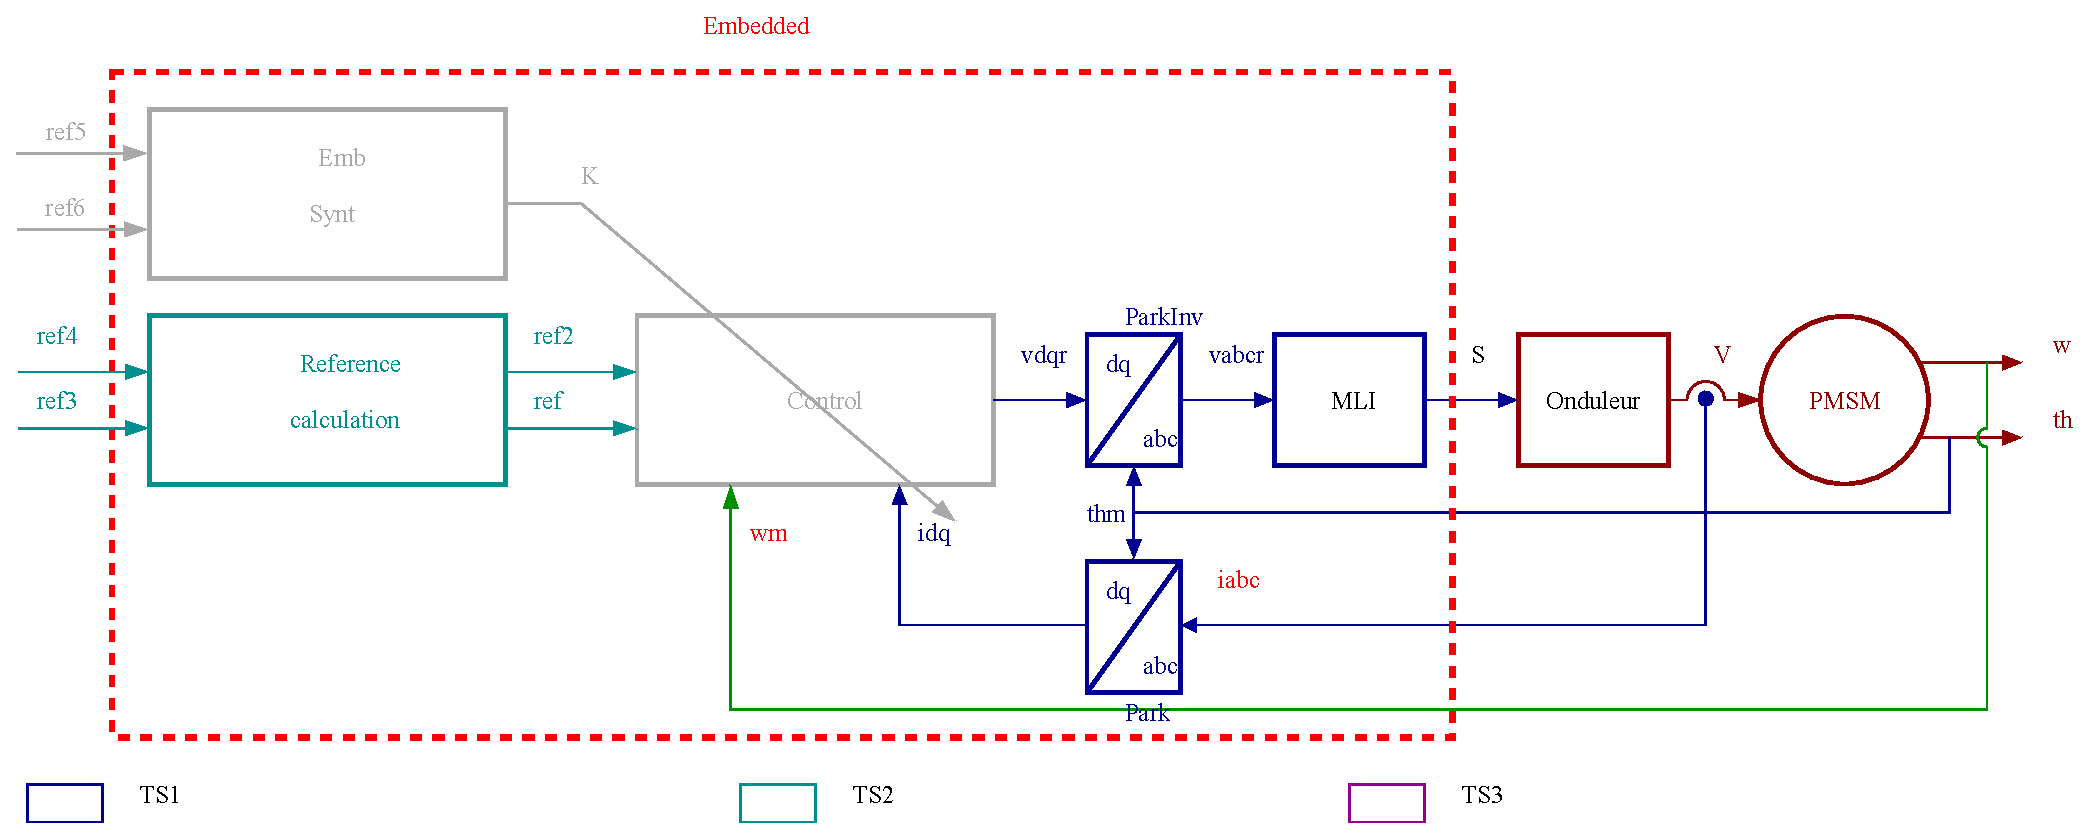
\includegraphics[width = .9\textwidth]{pictures/AdvancedControl_trajec.eps}
            \end{center}
        \label{fig:AdvancedControlForElectricalMotorTrajec}
        \end{figure}
\end{frame}
